\graphicspath{{./figures}}

\section{PocketQube Unit PCB}
Unfortunately, not enough prototypes were ready for an end-project University balloon launch. The power for the PQ unit was therefore implemented using large but readily available converters/regulators. In a final launch, however, this power section would either be replaced by the EPS, or a single, very low drop-out voltage regulator to convert the LiPo $\SI{3.7}{V}$ to a useable $\SI{3.3}{V}$.

The PQ unit PCB was ordered through an external supplier (JLCPCB). In order to begin initial development and testing, a breadboard prototype was initially created using an Arduino Nano, as shown in Appendix \ref{sec:appendix_pq}. Since the Nano has the same MCU as the designed PCB, the developed software could then simply be flashed onto the PQ unit using an off-board programmer.

The final module is shown in Figures \ref{fig:pqUnitPCB} and \ref{fig:pqUnitPower}. As noted in the errata in Appendix \ref{sec:appendix_pcb_errata}, the crystal's loading capacitors were mistakingly left out. The MCU's internal 8 MHz clock was therefore used. This clock, however, is generally badly calibrated, and resulted in software serial communication with the GPS module initially not working. This was fixed by setting the OSCCAL register in software to calibrate the clock.

\begin{figure}[!htb]
  \begin{minipage}{.49\textwidth}
    \centering
    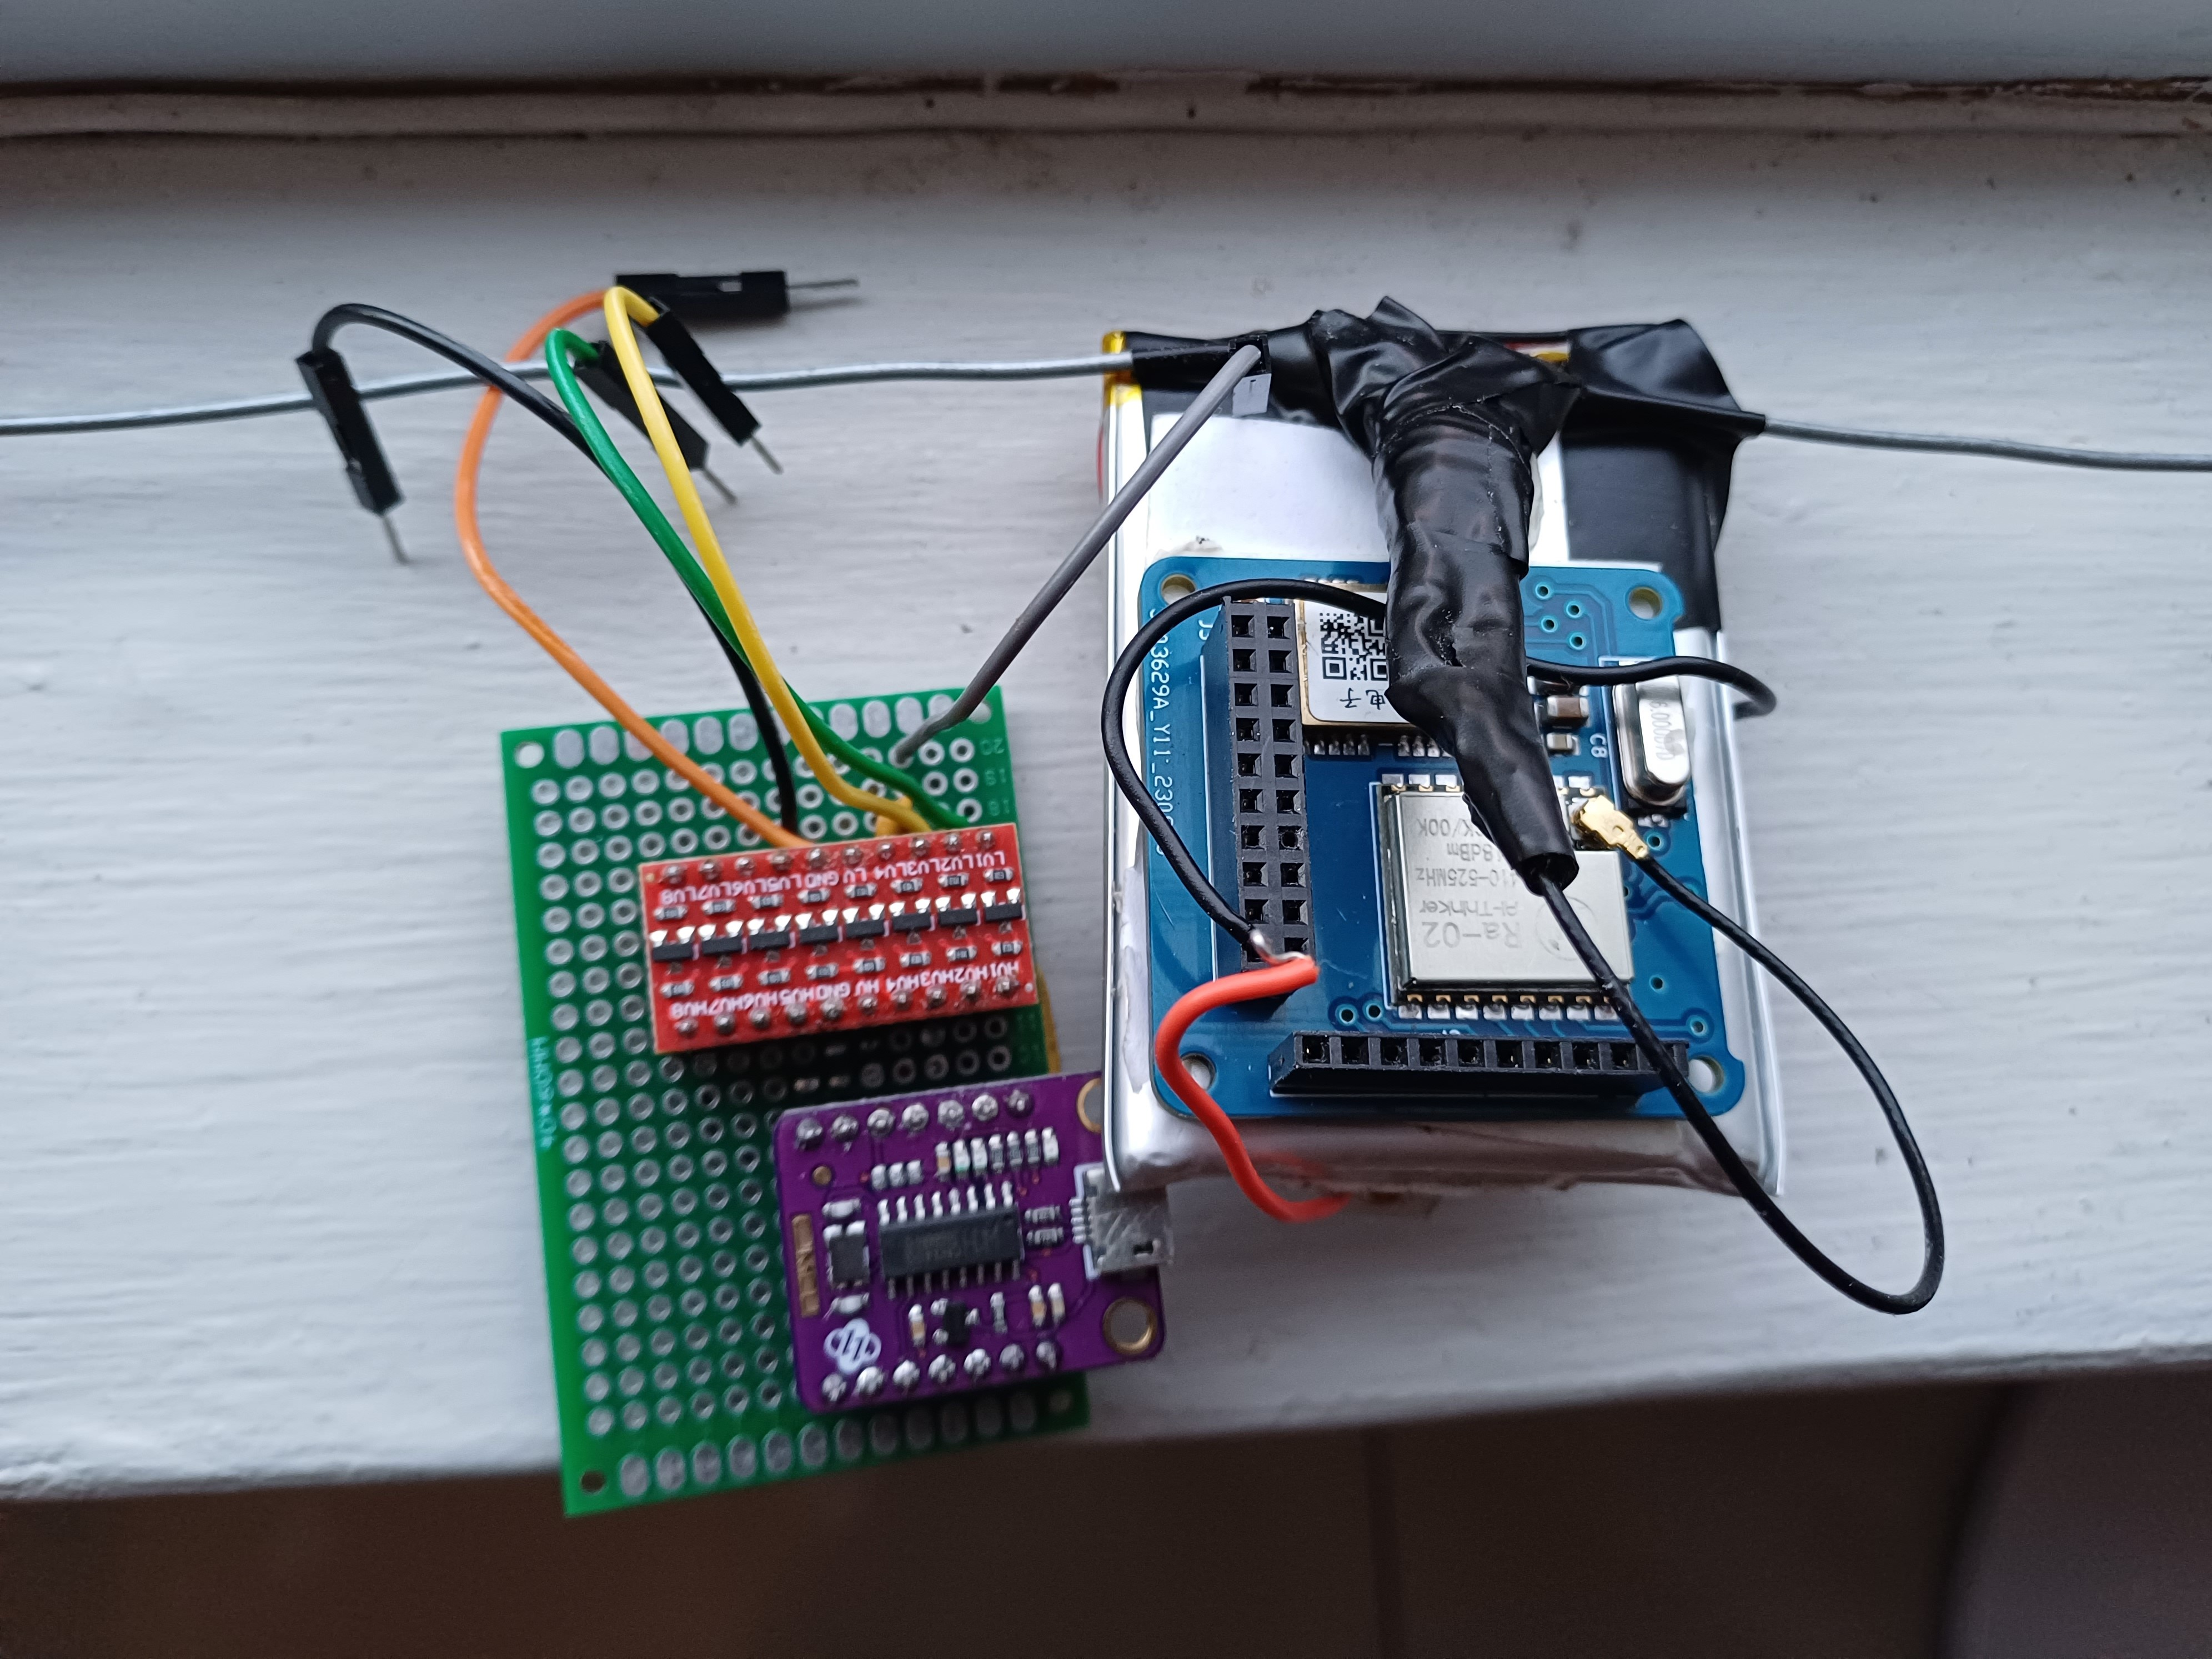
\includegraphics[width=0.85\linewidth]{pqUnitPCB}
    \caption{PQ Unit (front) [right] and programmer [left]}
    \label{fig:pqUnitPCB}
  \end{minipage}
  \begin{minipage}{.49\textwidth}
    \centering
    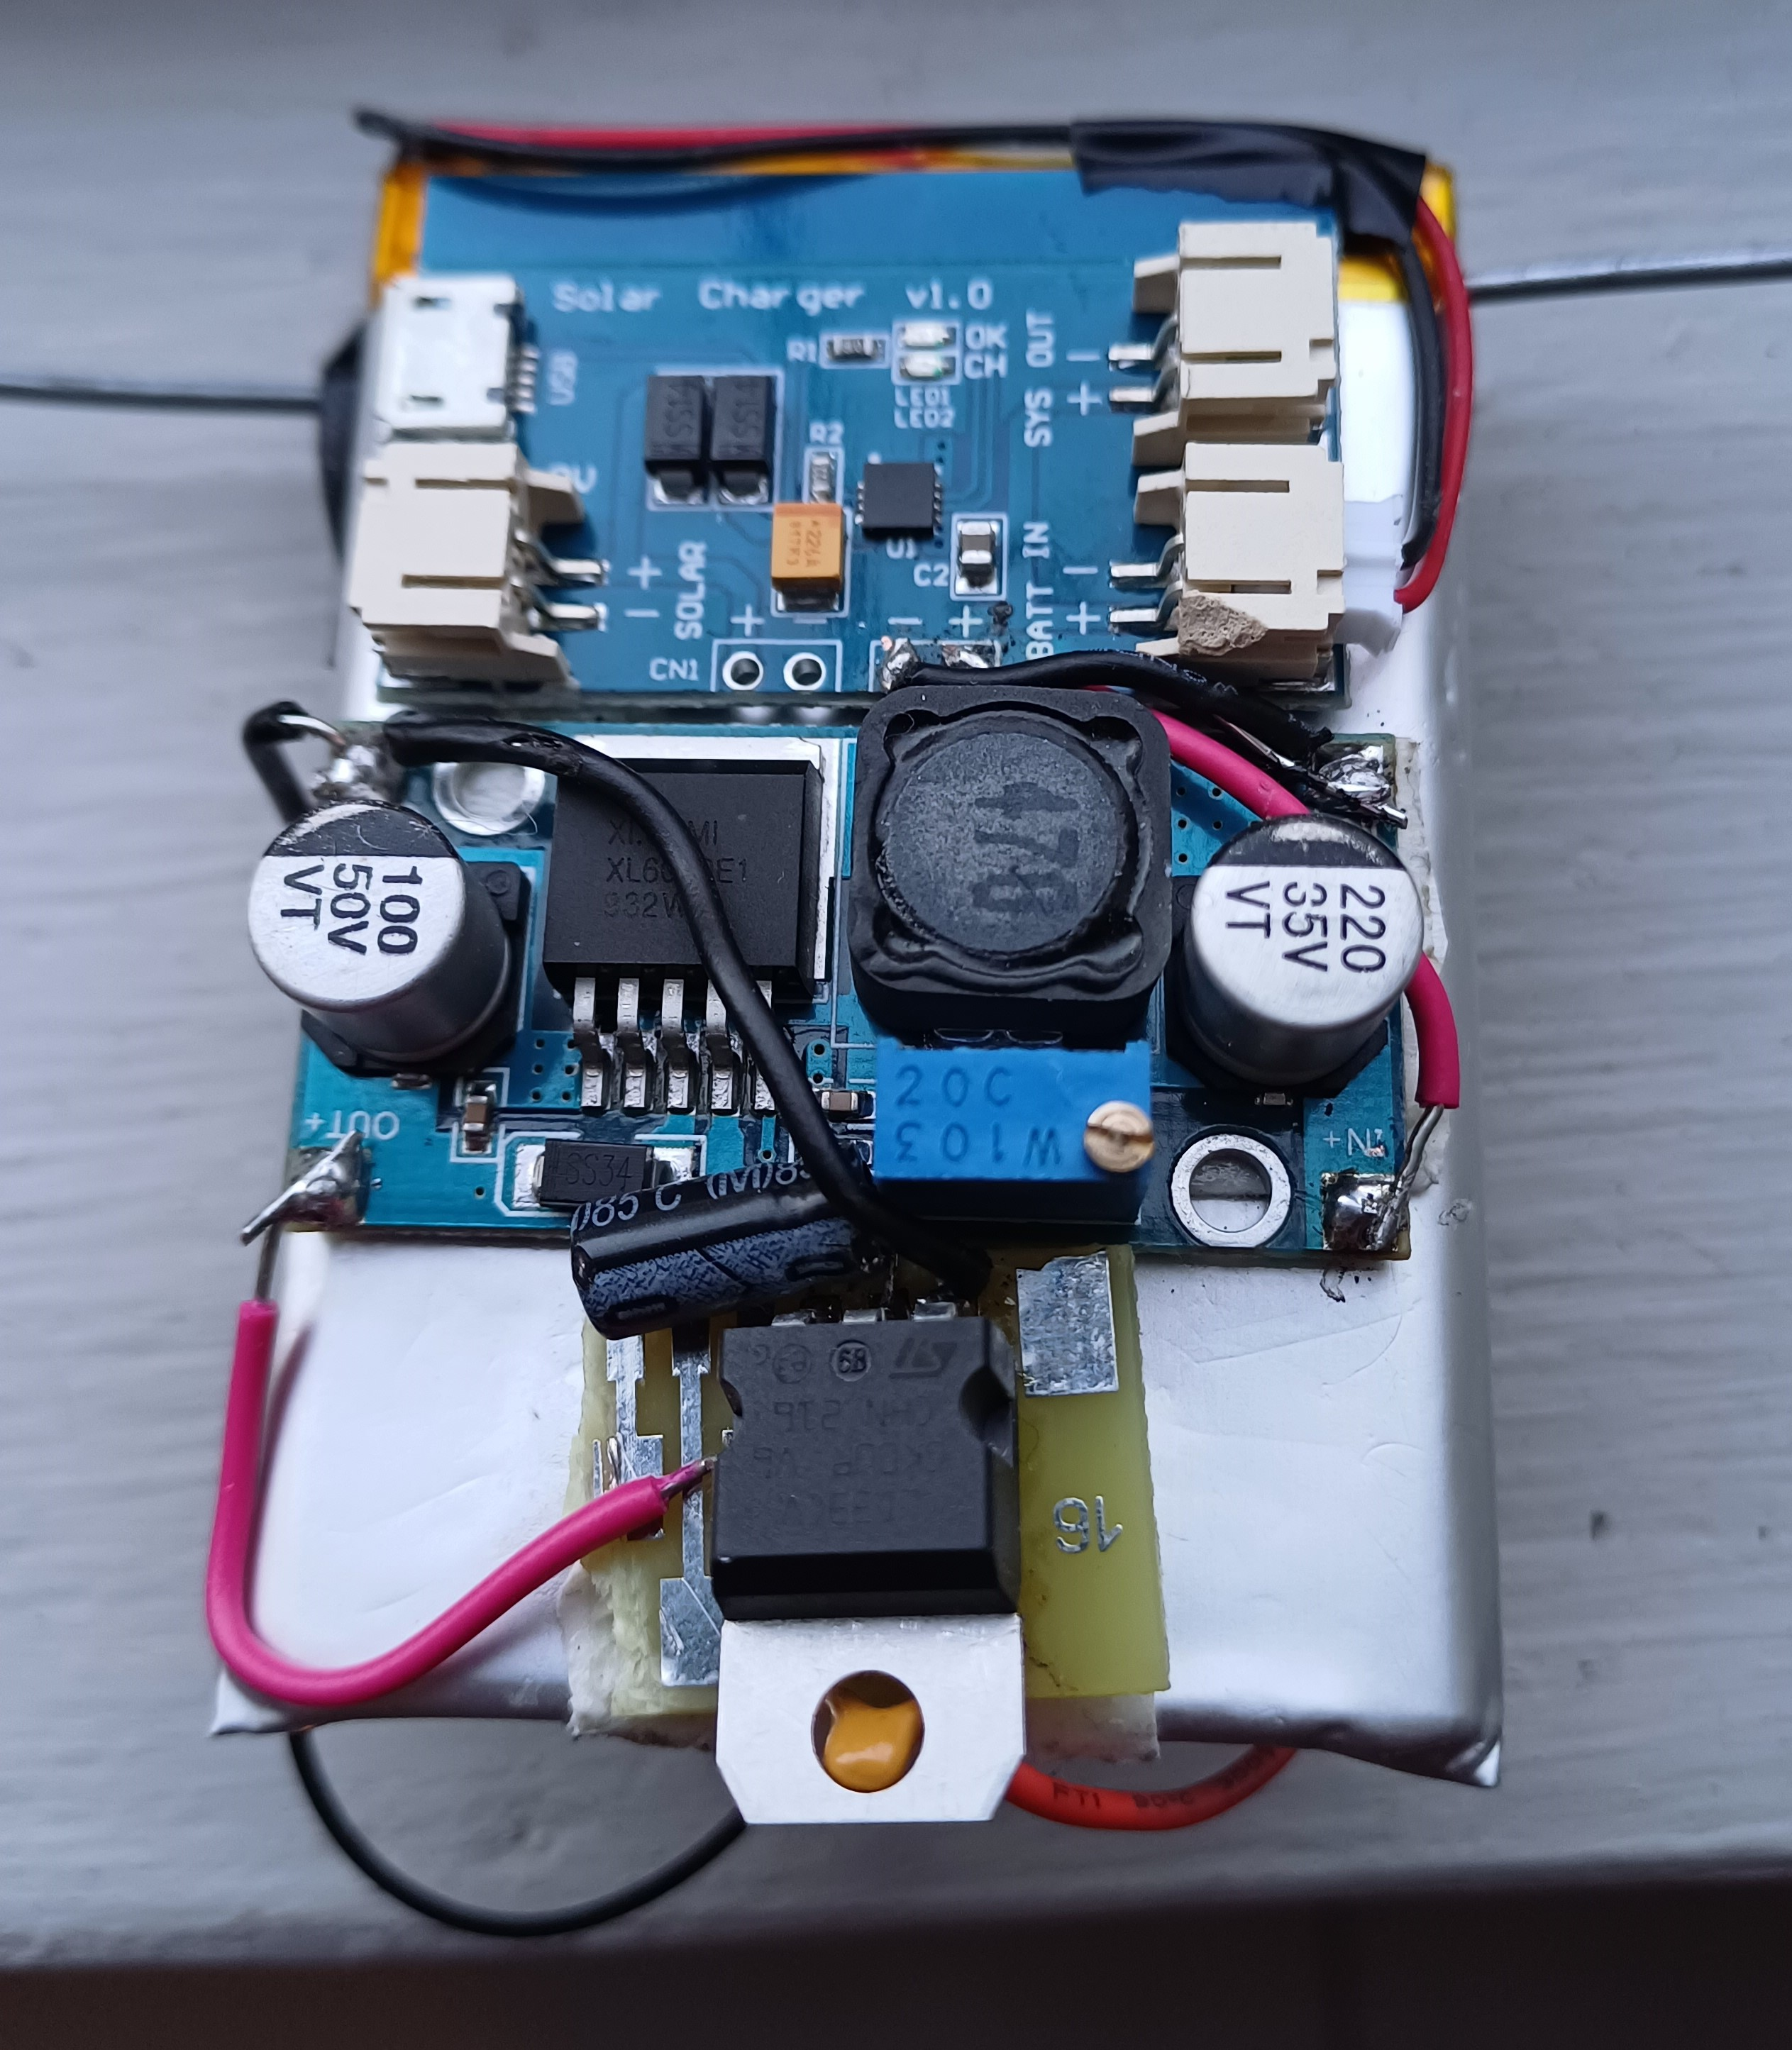
\includegraphics[width=0.6\linewidth]{pqUnitPower}
    \caption{PQ Unit (back)}
    \label{fig:pqUnitPower}
  \end{minipage}
\end{figure}

The board was first bootloaded with an Arduino Nano, and then the programmer circuit in Figure \ref{fig:pqUnitPCB} was developed to flash the board via UART. The programmer consists of a CH340 USB-to-serial module, a reset RC filter, as well as a 3.3V to 5V level converter (since the PocketQube PCB is designed to run at 3.3V). The board and dipole antenna was mounted onto the 2000 mAh LiPo battery. The power section consists of a LiPo charger, a boost converter module, and a 3.3V linear voltage regulator circuit.